%%Este capítulo debe ser el primer tema técnico a tratar,
%%debido a que mi tema se trata al modelado de objetos 
%%y de servicios de comunicación (al final los servicios
%%de comunicación se modelan como objetos via xml)
%%y también la utilización de interfaces da una buena base
%%para entender las capas del modelo OSI: las interfaces
%%que posee cada capa para comunicarse con las otras
%%(servicios) son muy bien compreendidas una vez
%%tratada el tema de interfaces de OOP. Al final, 
%%este tema de interfaces es 
%%abstracción, tratada en ingeniería de software. Por 
%%ello, es un buen punto empezar desde aquí.

\chapter{Object-oriented system construction}

\section{Introduction}

The IEC 61850 information model 
is classified as a  
\glsentrytext{O-O} system. Is necessary 
to have a clear understanding of \gls{O-O} technology
to dive into IEC 61850 object modelling. 
For this reason this chapter describes 
the \gls{O-O} technology
on which the IEC 61850 information model 
has been standarized\todo[inline]{No se si esta 
bien escrita la palabra standarized}. 

The chapter does not describe all the \gls{O-O} principles, 
just \todo{�trans:just focuses or focuses just?} focuses 
on the neccesary
background to understand the IEC 61850 
information model. 
The sections which follow will define the 
background which the IEC 61850 
object oriented information system 
was constructed, both formally 
and through examples.
\todo[inline]{debo agregar las abreviaciones de O-O
a mi glossaries package}
A detailed description of the \gls{O-O} fundamentals  
and reference materials are provided. To achieve a 
robust concepts comprehension a practical 
implementation with the%the Unified Modeling Language 
\gls{UML} 
\todo{agregar al glossaries} 
\cite{UML2:2009} 
and Java \cite{Java:specification} are provided. 
This chapter is very
practical in the sense that uses language programmings to model 
very carefully selected models  
used by the IEC 61850 standard, 
(but not explaining explicitly nothing 
about the standard yet!).
This chapter is destined 
for electrical engineers and professionals of 
related areas readers which the \gls{O-O} software construction 
is not part of the curriculum. For this reason, 
the practical examples uses electricity area 
elements. The readers with a strong knowledge 
of programming could skip this
chapter \todo[inline, color=blue!50!red!50]{
	deber\'ia agregar esta ultima frase?:
	\emph{The readers with a strong knowledge 
	of programming could skip this
	chapter}
}




\todo[inline]{En este cap�tulo voy a agregar 
los graficos a continuacion:

(los ejemplos que voy usando son con estas clases)}


\begin{figure}
  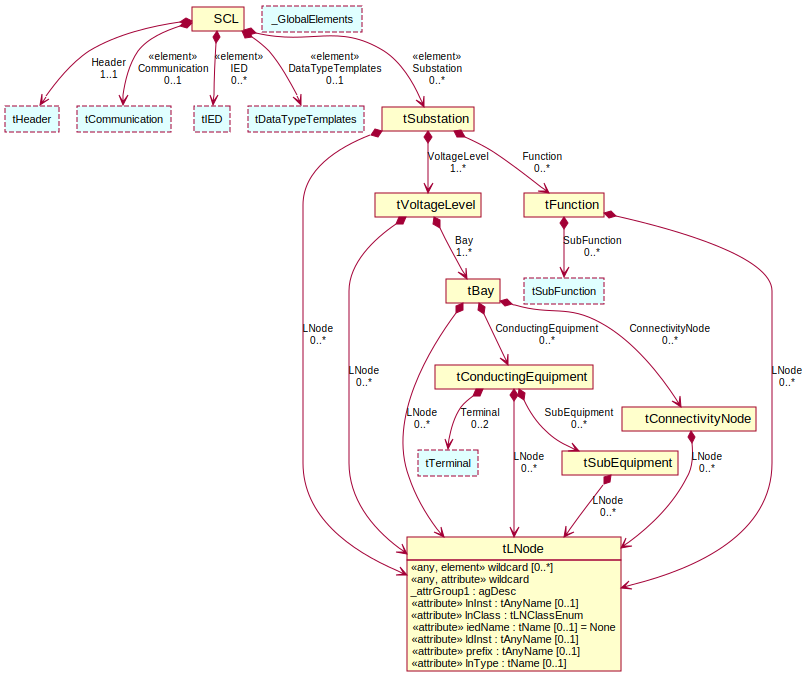
\includegraphics[width=1.0\textwidth]{chapters/ch-oop/figures/LogicalNodeAllocationStructure}
  \caption{Logical Node and their role at the substation level}
  \label{fig:LogicalNodeAllocationStructure}
\end{figure}

\begin{landscape}
	\begin{figure}	
	  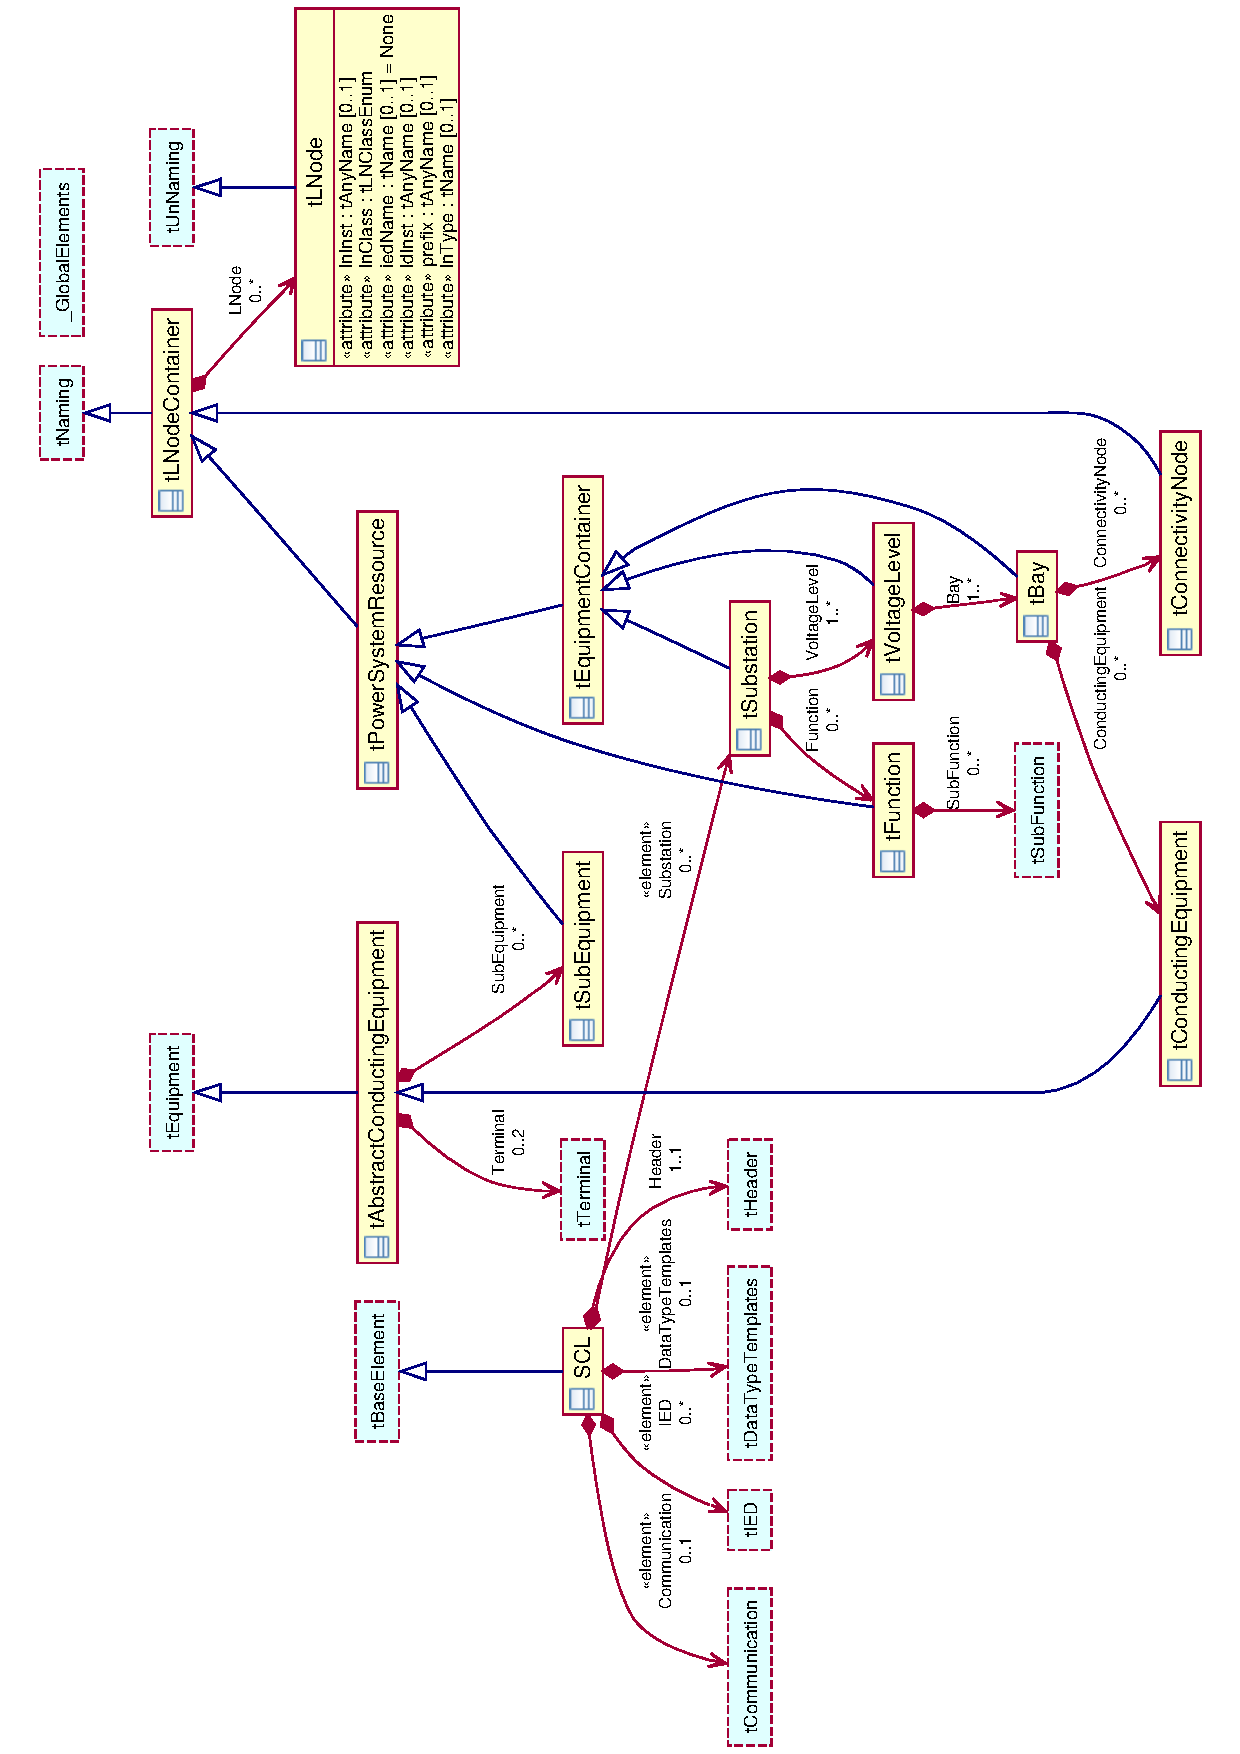
\includegraphics[angle=-90, width=1.0\linewidth]{chapters/ch-oop/figures/LogicalNodeAllocationStructure_with_heritance}
	  \caption{Logical Node and their role at the substation level, depicted with
	  the heritance details}
	  \label{fig:LogicalNodeAllocationStructure_with_heritance}
	\end{figure}
\end{landscape}
	
\section{Object Oriented systems}


%\todo[inline]{leer el paper de historia de poo, en la 2da pagina}
%\cite{Wegner:1987}

Many autors formulate precise 
definition of \gls{O-O} paradigm 
\cite{Rentsch:1982} 
\cite{Pascoe:1986}
\cite{Nygaard:1986}
\cite{Madsen:1988}, 
and the definition of Lastly, Wegner 
\cite{Wegner:1987} has been 
the most widely 
accepted \cite{Capretz:2003}. Wegner defines 
the \gls{O-O} paradigm in terms of objects, 
classes and inheritance.

\emph{
	``Objects are autonomous entities 
	that respond to messages or operations and share 
	a state. Classes classify objects by their common 
	operations. Inheritance serves to classify classes by 
	their shared behavior. Data abstraction hides the 
	representation of data and the implementation of 
	operations'' 
}\cite{Wegner:1987}. That is: 

\begin{center}
	object oriented = objects + classes + inheritance
\end{center}
In the next sections theses concepts are explained.

%This paradigm is useful to develop scalable, 
%consistent and reliable software systems 
%organizing the code to create objects. 
The O-O system programming metodology 
defines an approach to code organization 
for objects creation. 
The objects store the data and 
have their own behabiour with a 
particular information grouping 
by common functionality and common 
information structures. 
O-O systems benefits 
to bundle actions together, 
manage a few quantity of variables rather 
than multiples ones, 
organizing the 
common behavior together and 
structure programs in a way that
matches closely 
the real world \cite{Adobe:AS3man2008}. 

The figure \ref{fig:real-world-objets-represented} shows  
\todo{
	esta figura esta incompleta, deberia conseguir unas
	buenas fotos (en itaipu hay muchas fotos lindas y 
	originales) de estos equipamientos
	electricos de la Itaipu y colocar unas 
	flechitas que unen a estos 
	diagramas con los objetos reales
	y palabras indicativas\ldots
} 
a real world substation, their equipments, 
and the virtual substation  
software engineering representation 
through the class \emph{tSubstation} that 
responds with the same behabiour as in 
the real world, 
but running by software.


\begin{figure}
  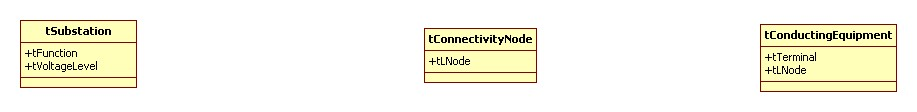
\includegraphics[width=1.0\textwidth]{chapters/ch-oop/figures/real-word-objets-represented}
  \caption{Real world object and their representation in software engineering}
  \label{fig:real-world-objets-represented}
\end{figure}


\section{Classes}

A class is a static 
%off-line \todo{es realmente off-line?}
template from which objects are 
created. Classes are used 
to classify objects thanks 
that its defines 
common operations 
and a data structure, 
and the types of 
datas that the object can 
store.\\


%Codigo fuente
%C:\Documents and Settings\DELL\Mis
%documentos\tesismayo\tesismayo\thesis\chapters\ch-oop\source\java\src\HelloWorld.java
%\lstinputlisting[label=samplecode,caption=A sample]{sourceCode/HelloWorld.java}
%chapters\ch-oop\source\java\src\HelloWorld.java
\lstinputlisting[label=codeClass,
caption=Class in Java]{chapters/ch-oop/source/java/src/SERVER_v1.java}

%%TODO: cite adobe book

\subsection{Attributes}
\todo[inline]{completar esta parte}
	\lstinputlisting[label=codeAttributes,
	caption=Class with attributes in Java]
	{chapters/ch-oop/source/java/src/SERVER_v2.java}



\subsection{Methods}
Methods are functions that are part of a class 
definition. Once an instance of the class is created, 
a method is bound to that instance.\\
	\lstinputlisting[label=codeMethod,
	caption=Class with attributes and methods in Java]
	{chapters/ch-oop/source/java/src/SERVER_v3.java}



	\subsubsection{Get and set accessor methods}
	Get and set accessor functions, also called getters 
	and setters, allow you to adhere to the programming principles of 
	information hiding and encapsulation while providing an 
	easy-to-use programming interface for the classes that you 
	create. Get and set functions allow you to keep your class 
	properties private to the class, but allow users of your class 
	to access those properties as if they were accessing a 
	class variable instead of calling a class method. 
	The advantage of this approach is that you can avoid 
	having two public-facing functions for each property 
	that allows both read and write access. \\

		\lstinputlisting[label=codeMethod,
		caption=Class with attributes, methods, getters and setters in Java]
		{chapters/ch-oop/source/java/src/SERVER_v4.java}
	
	
	\subsubsection{Constructor methods}
	Constructor methods, sometimes simply called constructors, 
	are functions that share the same name as the class in 
	which they are defined. Any code that you include in 
	a constructor method is executed whenever an instance of the 
	class is created with the  new  keyword. \\

		\lstinputlisting[label=codeMethod,
		caption=Class with attributes, methods, 
		getters, setters and constructors in
		Java] {chapters/ch-oop/source/java/src/SERVER_v5.java}

	
\section{Objects}

A object is a agrupation 
of datas and operations 
with autonomous memory 
which should inside 
in the behabiour of each invocation. 
The object datas have a state that remember 
the effect of the 
operation \cite{Wegner:1987}.
and unlike a class, a object  
just exist on a running proccess.
 
A object are created from a 
class, in other words, 
a object is a instance of a class.


A O-O program interaction 
is realized by 
objects invoking methods. 

	\subsection{Instance}
		\todo[inline]{por completar
			podrian servir como referencia los 
			siguientes links
			(antes debo verificar si estan bien):
			http://www.geekinterview.com/question_details/35271
			http://www.geekinterview.com/question_details/17747
		}
	
	
	
	\subsection{Reference}
	
	

\section{Diference betwen Classes and Objects}

They are a clear separation between 
class and object, 
and they are (together with inheritance) 
the most important concepts of O-O programming 
languages \cite{Dahl:1970}. 
%this separation was fist introduced by Simula 
%to simulate real-world applications. 

A class is a static off-line 
template to generate objects. 
A object is a runtime data 
or a group of datas 
according to the class. The objects are 
independend datas with 
its own behavior, and 
they are classified by the classes 
\todo{ESP:por las clases q la han generado}
which generated.


\input{chapters/ch-oop/inheritance}
\section{Information hidding and encapsulation}

	\section{Abstract data types}

Abstraction and information hidding form 
the foundation of all object-oriented 
development \cite{Levy:1984}. 
An abstraction is a simplified description, 
or specification, of a system that emphasizes 
some of the system's details or properties while
suppressing others \cite{Shaw:1984}.
Information hidding, as first promoted by Parnas,
\todo{explicar mas c/mis palabras} 
goes on to suggest that we should decompose 
systems based upon the principle of hidding 
design decisions about our 
abstractions \cite{Parnas:1979} \cite{Grady:1995}.

The abstraction and information hidding 
are very common in electrical equipments and 
mathematical representations of the 
electrical world. The 
models are abstracted 
and is possible to identify object and 
operations that exist at each level of integrations 
Thus, 
when \todo[inline]{ver si las palabras estan 
bien escritas en este ejemplo} we work 
with phasors to represent a current, which 
leave just the static amplitude and phase
information. The time space are hidden with 
the purpose to manage the information 
at a more hight level, 
thereby skipping the trigonometric calculations 
derived from the time dependence of the sine wave, 
and the information are combined just algebraically, 
simplifying certain kinds of complex 
calculations.  \cite{Grady:1995}

The abstraction  and information hidding are common 
in our activities, we abstract the models by 
identify the object and operations that exist 
at each level of integration. Thus, when
\cite[inline]{ver si las palabras estan 
bien escritas en este ejemplo} 
working a transformer, we consider the 
taps, the current on the low and hight side, 
the transformation relation \cite{Grady:1995}.

The use of abstract data types on a object oriented system 
help to a more precise and at the same time simple on the 
specification taking adventage of the information hidding 
provided by abstract 
data types. \cite{} \todo{aca debo citar mi paper sobre ACSI}





	\section{Intefaces}

%\input{chapters/ch-oop/blah blah blah}

	\subsection{Encapsulation}

The encapsulation is a technique for 
avoid dependencies among 
classes and modules by defining 
strict interfaces, and 
help for software 
maintenance, 
by information hidding,
understandability of code, 
localization of information,
narrow interfaces,  
and information restriction \cite{Lieberherr:1988}. 
%difference of information hidding 
%and information restriction are explained
%by the law of demeter paper Lieberherr:1988.



	\section{Interfaces and implementation}

\todo[inline]{modificar, reelaborar con mis palabras}

Interfaces are based on the distinction between a 
methods interface and its implementation. A method’s interface 
includes all the information necessary to invoke that 
method, including the name of the method, all of its 
parameters, and its return type. A method’s 
implementation includes not only the interface 
information, but also the executable statements 
that carry out the method’s behavior. An 
interface definition contains only method 
interfaces, and any class that implements 
the interface is responsible for defining the 
method implementations. 
%%TODO: falta explicar más, enfocando desde 
%%el punto de vista de ingeniería de software
\cite[pp.~90-105]{Adobe:AS3man2008}

\todo[inline]{agregar aca lo que subraye
y resum� en
la segunda pagina del paper snyder:1986}	

\section{Object oriented develoment approach}

The object-oriented development should 
follow the steps proposed by Aboott \cite{Abbott:1980}:  

\begin{itemize}
  \item Identify the objects and their attributes.
  \item Identify the operations suffered by and required
		of each object.
  \item Establish the visibility of each object in 
		relation to other objects.
  \item Establish the interface of each object.
  \item Implement each object.  
\end{itemize}


